\documentclass[landscape,archE,fontscale=0.285]{baposter}

\usepackage{graphicx} % Required for including images
\graphicspath{{figures/}} % Directory in which figures are stored

\usepackage{amsmath}
\usepackage{amssymb}

\usepackage{url}
\usepackage{listings}

\usepackage{booktabs} % Top and bottom rules for tables
\usepackage{enumitem} % Used to reduce itemize/enumerate spacing

\usepackage[font=small,labelfont=bf]{caption} % Required for specifying captions to tables and figures

\usepackage{multicol} % Required for multiple columns
\setlength{\columnsep}{1.5em} % Slightly increase the space between columns
\setlength{\columnseprule}{0mm} % No horizontal rule between columns

\definecolor{lightblue}{rgb}{0.145,0.6666,1} % Defines the color used for content box headers

\newcommand{\compresslist}{ % Define a command to reduce spacing within itemize/enumerate environments, this is used right after \begin{itemize} or \begin{enumerate}
\setlength{\itemsep}{1pt}
\setlength{\parskip}{0pt}
\setlength{\parsep}{0pt}
}

\usepackage[
backend = biber,
style = numeric
]{biblatex}
\addbibresource{final.bib}

\renewcommand*{\bibfont}{\tiny}

\begin{document}
\begin{poster}
{
eyecatcher = false,
background = none,
headerfont=\Large\bf\textsc, % Large, bold and sans serif font in the headers of content boxes
headerheight=0.1\textheight, % Height of the header
headershape=roundedleft, % Specify the rounded corner in the content box headers, can be: rectangle, small-rounded, roundedright, roundedleft or rounded
headerColorOne=white, % Background color for the header in the content boxes (left side)
headerColorTwo=lightblue, % Background color for the header in the content boxes (right side)
boxColorOne=white, % Background color of the content boxes
borderColor=white
}
%----------------------------------------------------------------------------------------
%	TITLE SECTION 
%----------------------------------------------------------------------------------------
%
{
\includegraphics[height=4em]{logo.png}} % First university/lab logo on the left
{\bf\textsc{Chaotic Dynamics in Chua's Circuit}\vspace{0.5em}}
{\textsc{Jackson Dougherty }}
{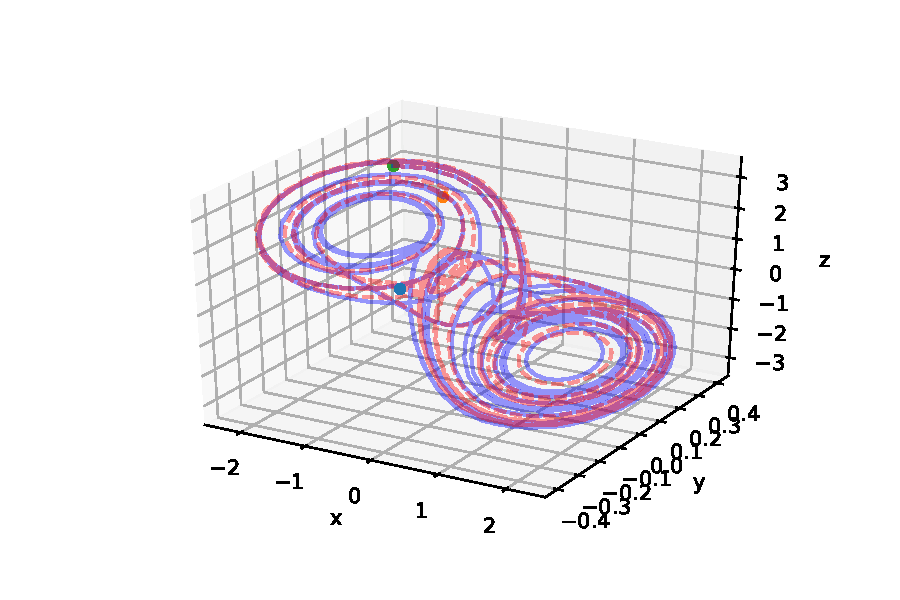
\includegraphics[height=10em]{twoAttractors.pdf}} % Second university/lab logo on the right

%----------------------------------------------------------------------------------------
%	INTRODUCTION
%----------------------------------------------------------------------------------------


%Chaotic Systems

\headerbox{Problem}{name=problem,column=0,row=0}{
In the early 20th century, mathematicians showed that some dynamical systems exhibit chaos; however, the study of chaotic systems became much more broadly interesting in the latter half of the century as scientists realized that many physical systems exhibit chaos and were able to demonstrate these dynamics using digital computers \cite{Solr-4807068}. By definition, chaos refers to the dynamical property that, as time evolves, initial conditions that are arbitrarily close together move exponentially far apart. Thus, as time passes, any error in the initial condition will grow exponentially, and the hypothesized trajectory will hold little value as a prediction of the system's future state. It is possible to estimate the rate of this exponential growth using a Lyapunov exponent. Strange attractors are defined as attractors with fractal dimension. Whereas a finite collection of points has dimension zero or a plane has dimension two, more complicated abstract sets can have fractional dimension. Chaotic systems often have strange attractors, and so we wish to characterize the dimension of a given attractor. 

\vspace{0.3em} % When there are two boxes, some whitespace may need to be added if the one on the right has more content
}

%----------------------------------------------------------------------------------------
%	RESULTS 1
%----------------------------------------------------------------------------------------

\headerbox{Chua's Circuit}{name=results,column=1,span=2,row=0}{


\begin{multicols}{2}
\begin{center}
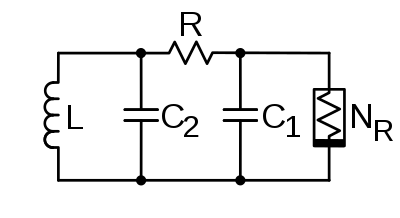
\includegraphics[width=0.8\linewidth]{Chua's_circuit}
\captionof{figure}{Schematic of Chua's circuit. Note that the circuit is not driven by any source. The nonlinear component $N_r$ leads to oscillations in the system. \cite{wiki:xxx} }
\label{image:ChuaCircuit}
\end{center}

Chua's circuit is a simple, autonomous, reciprocal circuit pictured in Fig. $\ref{image:ChuaCircuit}$. The only non-linear component, known as Chua's diode $N_r$, is piecewise linear. Such a circuit element is physically realizable, and exhibits chaotic dynamics \cite{edscal.902330719840101}. Indeed, a set of three ordinary differential equations, Eqs. $(\ref{1a})$, $(\ref{1b})$, and $(\ref{1c})$, models the system (See \cite{9284098519850108} and \cite{edseee.108586919860101} for the non-dimensionalization). 
\begin{align}
\frac{dx}{d\tau} &= \gamma(y-f(x)) \label{1a}\\
\frac{dy}{d\tau} &= x-y+z \label{1b} \\
\frac{dz}{d\tau} &= -\beta y \label{1c} 
\end{align} 

%------------------------------------------------

The nonlinearity in Eq.$\ref{1a}$ here takes the form $f(x)=G_b x + 0.5(G_a-G_b)(|x+1|-|x-1|)$, such that $E=1$ in Fig. $\ref{image:ChuaDiode}$. The parameters $(\gamma, \beta, G_a, G_b)$ are dependent upon the physical system, but for the discussion that follows, we will use $(9, 100/7, -1/7, 2/7)$. Physically, the variables $x$, $y$, and $z$ represent non-dimensional scaling of the voltage across the first capacitor $C_1$, the voltage across the second capacitor $C_2$, and the current through the inductor $L$. Time is likewise scaled to generate $\tau$.  

\begin{center}
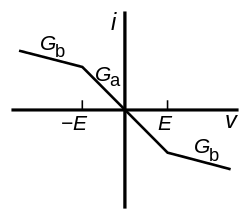
\includegraphics[width=0.8\linewidth]{Chua_diode}
\captionof{figure}{Characteristic curve for the diode $N_r$ in Chua's circuit. See Fig. $\ref{image:ChuaCircuit}$. \cite{wiki:xxx}}
\label{image:ChuaDiode}
\end{center}

\end{multicols}
}



%----------------------------------------------------------------------------------------
%	REFERENCES
%----------------------------------------------------------------------------------------

\headerbox{References}{name=references,column=0, span =2, above=bottom}{

\printbibliography[heading = none]
}

%----------------------------------------------------------------------------------------
%	FUTURE RESEARCH
%----------------------------------------------------------------------------------------

\headerbox{Future Research}{name=futureresearch,column=2,aligned=references,above=bottom}{ % This block is as tall as the references block

Additional effort could be devoted to developing more efficient algorithms for calculating the dimension. Even the fastest $\Theta(n^2)$ algorithm for calculating the correlation integral is still fairly slowly for $n=50000$, especially when calculated for ten different values of $\epsilon$. 
}

%----------------------------------------------------------------------------------------
%	CONTACT INFORMATION
%----------------------------------------------------------------------------------------

\headerbox{Contact Information}{name=contact,column=3,aligned=references,above=bottom}{ % This block is as tall as the references block

\begin{description}\compresslist
\item[Email] jackson.dougherty@uchicago.edu
\item[GitHub] https://github.com/jacksonDougherty/ PHYS250FinalProject.git
\end{description}
}

%----------------------------------------------------------------------------------------
%	CONCLUSION
%----------------------------------------------------------------------------------------
\headerbox{Conclusion}{name=conclusion,column=2,span=1,row=0,below=results,above=references}{

Determination of geometrical properties of the system is computationally intensive. A computation of the box count $\tilde{N}(0.01)$ with 500 points on the attractor with initial condition $(1.5,-0.2,-0.1)$ took over two hours. Ideally, closer to $50,000$ orbit points would be used to compute $\tilde{N}(\epsilon)$ for several small epsilon, and then the dimension $D_0$ could be found by regression. Likewise, $D_1$ and $D_2$ could be computed from their respective definitions, where $D_1 = \lim_{\epsilon\rightarrow0}\frac{\sum_{i=1}^{\tilde{N}(\epsilon)} \mu_i  \ln \mu_i }{\ln \epsilon}$ by L'Hopital's rule applied to the definition.

}

%----------------------------------------------------------------------------------------
%	MATERIALS AND METHODS
%----------------------------------------------------------------------------------------

\headerbox{Methods}{name=method,column=3,row=0,bottomaligned=problem}{ % This block's bottom aligns with the bottom of the conclusion block

The system of differential equations, $(\ref{1a})-(\ref{1c})$, was solved as an initial value problem using the \texttt{LSODA} solver from the \texttt{scipy.integrate} library. This ODE solver is described as 'a good universal choice' within the \texttt{scipy} documentation. Regression utilized the \texttt{scipy.optimize} library and a regression script from \cite{physLabWiki}. Additionally, the \texttt{numpy} and \texttt{matplotlib} libraries were used throughout to store, manipulate, and plot data. 

\begin{center}
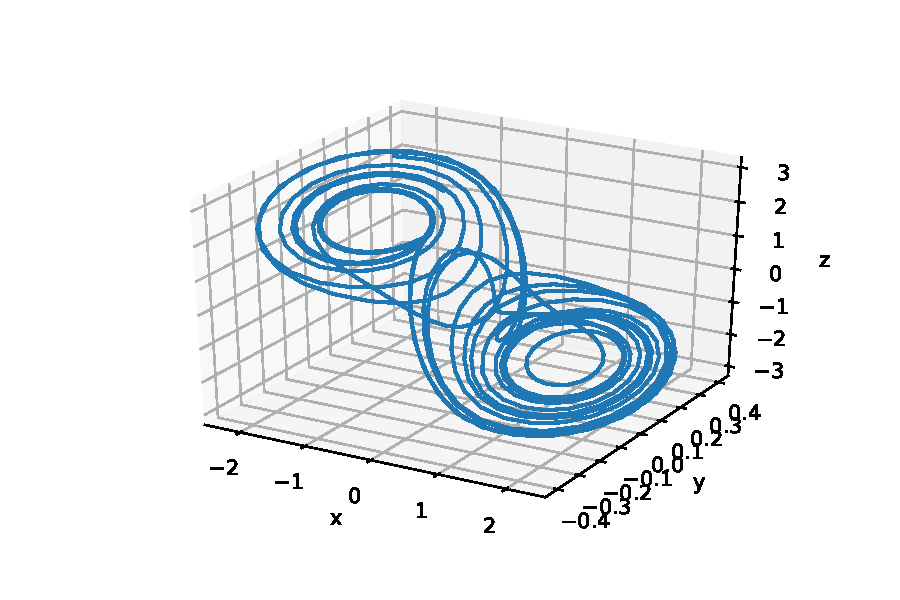
\includegraphics[width=0.8\linewidth]{ChaoticAttractor.pdf}
\captionof{figure}{Chaotic attractor generated by 500 time steps with initial condition $(x_0, y_0, z_0)=(1.5,-0.2,-0.1)$.}
\label{plot:chaosAttractor}
\end{center}

\begin{center}
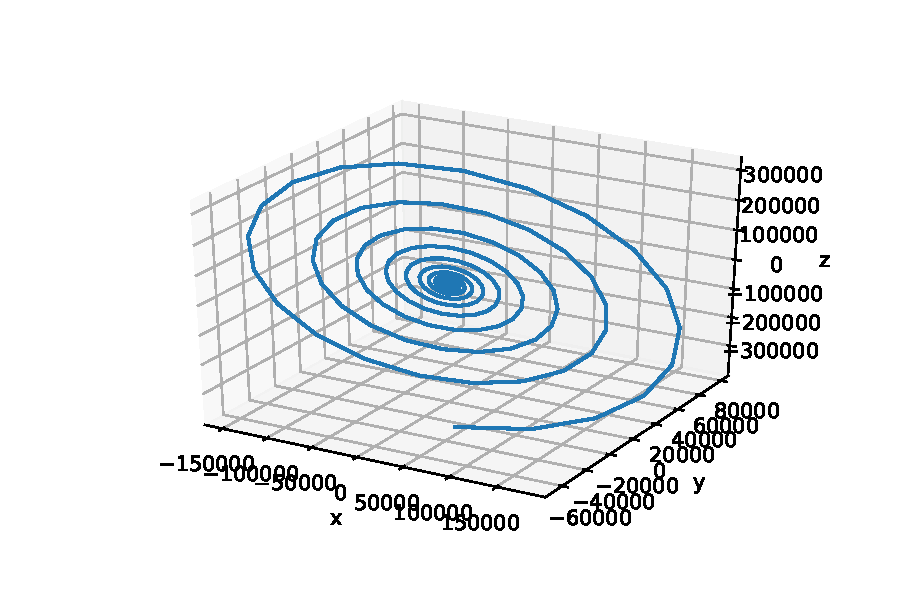
\includegraphics[width=0.8\linewidth]{UnstableAttractor.pdf}
\captionof{figure}{Unstable trajectory generated by 500 time steps with initial condition $(x_0, y_0, z_0)=(1.5,-0.2, 10)$.}
\label{plot:unstableTrajectory}
\end{center}
}
\headerbox{Dimension}{name=dimension,column=0,below=problem,bottomaligned=conclusion}{
There are several definitions of dimension characterize a set. The three considered here are defined on a spectrum, 
\begin{align}
D_q &= \frac{1}{1-q} \lim_{\epsilon\rightarrow 0}  \frac{\ln I(q, \epsilon)}{\ln(1/\epsilon}, \label{dim1} \\
I(q, \epsilon) &= \sum^{\tilde{N}(\epsilon)}_{i=1} \mu_i^q ,\label{dim2}\\
\mu_i  &= \lim_{T\rightarrow \infty} \frac{\eta(C_i, \bf{x}_0, T)}{T}, \label{measure}
\end{align}
where $\eta(C_i, \bf{x}_0,T)$ is the fraction of time that the orbit with initial condition spends in the $i$th cube $C_i$ between time $0\leq \tau \leq T$ and $\tilde{N}(\epsilon)$ is the number of cubes in a grid of size $\epsilon$ required to cover the attractor. \cite{Solr-4807068}

}
\headerbox{Dimension Interpretation}{name=interpretation,column=1,below=results,bottomaligned=conclusion}{
The box counting dimension $D_0$ may be interpreted using an approximation that follows from $I(0, \epsilon)=\tilde{N}(\epsilon)$, $\tilde{N}(\epsilon)\sim \epsilon^{-D_0}$.
The information dimension $D_1=\lim_{q\rightarrow1} D_q$ has the property that it agrees with the local dimension of the attractor almost everywhere, with respect to the measure $\mu$ defined in Eq. $(\ref{measure})$. 
Finally, the correlation dimension $D_2$ is simple to measure, and acts as a lower bound on the previous measures. $I(2, \epsilon)\sim C(\epsilon) = \lim_{K\rightarrow \infty} \frac{1}{K^2} \sum_{i,j}^{K} U(\epsilon - |\bf{z}_i - \bf{z}_j|)$, where the sum is computed over pairs $i,j$ of points $z_k$ in the orbit, and $U$ is the unit step function \cite{Solr-4807068}. 
}
\end{poster}
\end{document}